\documentclass[main.tex]{subfiles}

\begin{document}
\chapter{Detailed Design}
\chaplabel{detailedDesign}
The detailed design is a result of a more thorough design process, following the outcomes from the concept design, and will form the basis of the work programs for the project. This detail design will become the reference point for the construction and development during the build phase of the project, and has been selected as being a time effective and cost effective solution to delivering the project goals. The detailed design has been separated into subsystems which can be developed concurrently, maximising productivity of team members. These subsystems and their designs are detailed below.

\section{Navigation}
\seclabel{detailednav}
Platform navigation is primarily handled via waypoints. After a region is selected by a user it
is broken down into a series of waypoints which the quad bike will attempt to follow. In the
alternate use case, the user will specify a path directly and the navigation system will operate
directly on these waypoints.
\subsection{Waypoint Generation}
\seclabel{detailedwaypointgen}
The waypoints are generated from a zone of interest to facilitate the autonomous surveying of areas that are suspected to contain mines. This zone must be capable of being user defined to match real world boundaries. The algorithm used to generate these waypoints is a modified linescan algorithm which will be tuned to output scanlines of the same width as the equipment's scan width.

To allow for complex polygonal zones to be entered by the user, the original user-defined polygon boundary is split into a series of convex hulls, simplifying the line scanning algorithm. The split of the user polygon is shown in \Figref{wayPointGeneration}, where the user-defined polygon is outlined in bold blue and the series of generated convex search regions are shaded within. The black path shows the output of the linescan algorithm starting at the origin (marked by the red dot in the south-east corner), and ends at the second red dot at the far end of the path. The linescan algorithm searches for the nearest corner from the nearest convex polygon and begins plotting successive alternating scanlines through the polygon. After a convex polygon has been completely covered, the linescan algorithm connects to the next nearest corner of the next nearest polygon and the process continues. This system allows for multiple user defined regions to be connected and autonomously scanned in a single pass.

\begin{figure}[ht]
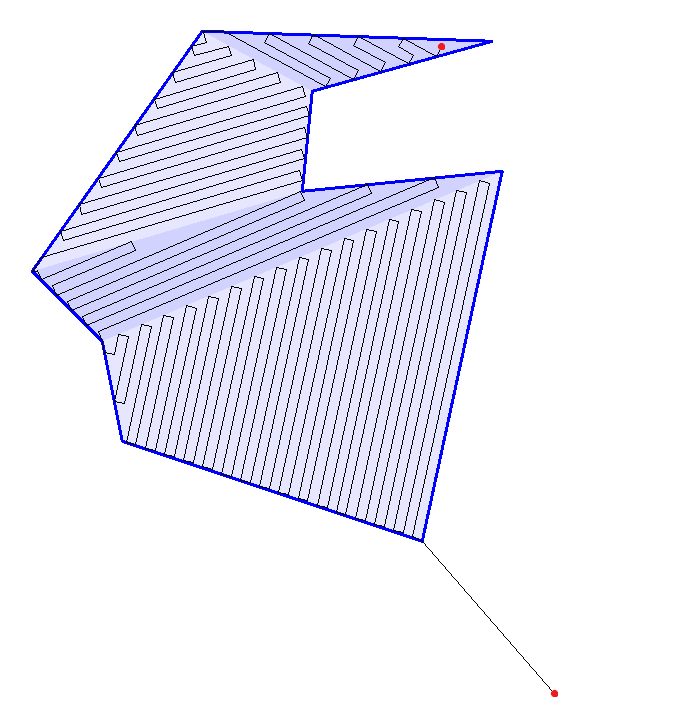
\includegraphics[width=0.5\textwidth]{5-DetailedDesign/lineScanAlgorithm.png}
\centering
\caption{Output of preliminary waypoint generation algorithm} \figlabel{wayPointGeneration}
\end{figure}

\subsection{Low Curvature Path Following}
For low curvature path following (such as a straight line connecting waypoints discussed in \secref{detailedwaypointgen}) Pure Pursuit is used. The tracker works through determining an arc that connects the non steering wheel axle to a goal point on the path (refer back to \Figref{purePursuitGeom}).  The goal point ($g_x, g_y$) acts as an intermediate waypoint and is determined from a look-ahead distance $l_d$. The angle, $\alpha$, can be related to the geometry using the law of sines,
\begin{align*}
\frac{l_d}{\sin(2\alpha)} &= \frac{R}{\sin(^{\pi}/_2-\alpha)},\\
\frac{l_d}{2\sin(\alpha)\cos(\alpha)} &= \frac{R}{\cos(\alpha)},\\
\frac{l_d}{2\sin(\alpha)} &= R.
\end{align*}
Then the steer angle, $\delta$, can be determined from the geometry shown in \Figref{geometricBicycleModel} where
\begin{figure}[ht]
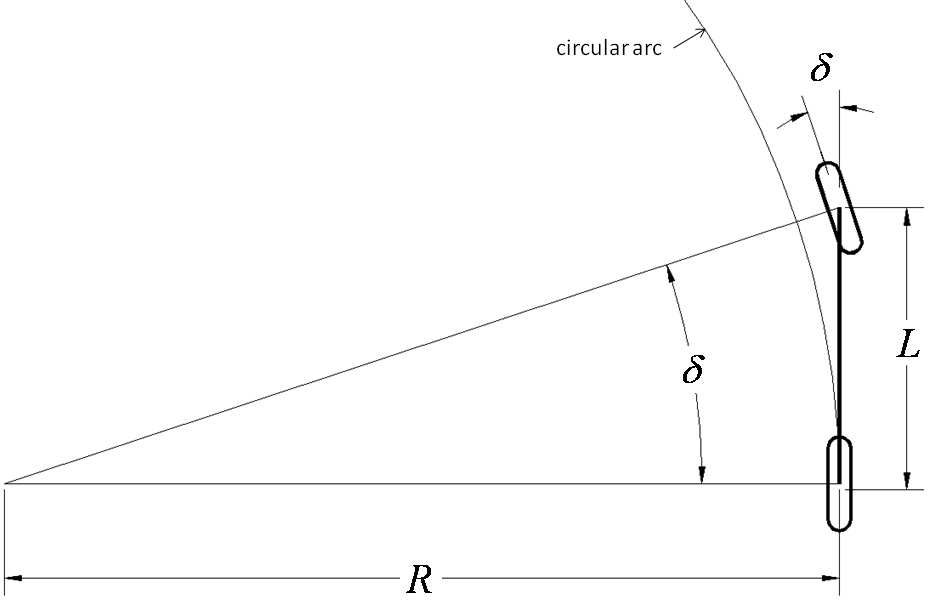
\includegraphics[width=0.7\textwidth]{5-DetailedDesign/Geometric_Bicycle_Model.png}
\centering
\caption{Geometric bicycle model} \figlabel{geometricBicycleModel}
\end{figure} 
\begin{align*}
R &= \frac{l_d}{2\sin(\alpha)},
\shortintertext{and the pure pursuit controller is given as}
\delta &= \tan^{-1}\Bigg(\frac{2L\sin(\alpha)}{l_d}\Bigg)
\end{align*}
where $\alpha$ and thus $\delta$ will be functions of time (calculated in real time in practice).
A separate algorithm is used for turning a specified angle due to real quad bike geometry where a minimum turn radius is introduced.
\subsection{Turning the Platform a Specified Angle}
It is evident from \Figref{wayPointGeneration} that many sudden and sharp turns will be encountered during the navigation process. If the quad bike is not to stray a great distance from the path, the pure pursuit method breaks down due to turn angle limitations on the quad bike.  In these situations an alternate method will need to be processed in the code to turn the quad bike the required angle while not leaving a scanned region (governed by the width of the detection array). One solution is to conduct an N-point turn within the swathe which is achieved through placing waypoints at each of the end turn points.

\section{Sensor Mount}
Both the GPR and metal detector are required to be mounted to the platform in a cantilever-like fashion in order to avoid contact with the ground where it would risk detonation of a landmine. Each of the sensor arrays is expected to weigh between 10 kg and 30 kg.
Mounting needs to be done in a configuration that will keep individual array sensors aligned so that corresponding ground information can be collated and analysed correctly. If the assumption of Ackermann steering holds for the quad bike we can use the simplified, 2-wheel model to assess the location of the sensors relative to the quad bike. The simplified model provides the following geometric relationship:
$$
tan(\delta) = \frac{L}{R}
$$
Where $\delta$ is the steering angle, $L$ is the wheelbase and $R$ is the radius of the arc that the centre of the rear axle will follow. This simplification has been used to perform simulations on the steering effectiveness of the vehicle and will also be used to estimate turning capabilities as part of the route planning software.
Initial simulations showed that front mounted sensors with rear-wheel steering is the best option for the application with far superior coverage results compared to front-wheel steering. Further results are shown in \Figref{turnCoverage}
\begin{itemize}
\item Trial 1, represented as the leftmost diagram in \Figref{turnCoverage}, shows the turning example for a case where the turning wheels are 1.5 metres in front of the focal point of the turn, or front wheel steering. The sensor array is 0.5 metres in front of the turning wheels, 2 metres from the focal point of the turn. Evident from the figure is how the coverage area does not form a tight loop and the coverage area does not include the path of the vehicle. This is critical as it will mean the quad bike will be passing over ground not scanned by the sensors.
\item Trial 2, represented by the middle diagram in \Figref{turnCoverage}, shows the results for a case where the turning wheels are 1.5 metres behind the focal point of the turn, or rear wheel steering. The sensor array is placed 0.5 metres in front of the focal axle. This trial shows a much tighter scanning loop than the previous test and the path of the quad bike is entirely within the scanned area. This is ideal.
\item The third trial, represented by the rightmost diagram in \Figref{turnCoverage}, is purely for comparison and shows the coverage area of a vehicle with turning wheels 1.5 metres in front of the focal axle, but with the sensing array only 0.5 metres in front of the focal axle. This would place the sensing array between the two axles of the vehicle. Under this arrangement an identical scanning path is achieved using a front-wheel steering setup. This is not useful for the application as the sensors must be in front of the vehicle to detect landmines.
\end{itemize}
% Split, subfig
\begin{figure}[ht]
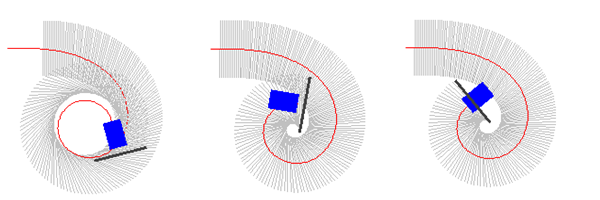
\includegraphics[width=0.8\textwidth]{5-DetailedDesign/Detector_Coverage.png}
\centering
\caption{Mine detector coverage simulations} \figlabel{turnCoverage}
\end{figure}
This result is expected. Referring to \Figref{geometricBicycleModel}, the turning radius of the rear wheel is $R$ and the turning radius of the front wheel is the hypotenuse of the triangle formed – of length $\sqrt{R^2 + L^2}$, which is greater than $R$. If the sensing array was some distance $q$ in front of the front wheels, its turning radius would be $\sqrt{R^2 + [L+q]^2}$, greater yet again. However, if the sensing array was an equal distance $q$ behind the rear wheels (or front wheels if this was a rear-steering arrangement) then the turning radius of the sensors would be $\sqrt{R^2 + q^2}$. From this it can be seen that to minimise the effective turning radius then $q$ should be minimised.

The sensor arrays will be mounted at the 'rear' of the quad bike which will be primarily driven in reverse to achieve the desired scan coverage. The mounting bracket for the arrays will be constructed on-the-fly with the assistance of the workshop and its technicians. The bracket should be constructed from PVC and meet the following specifications:
\begin{itemize}
\item Metal detector clear of metal in a 500 mm radius and 2000 mm vertically.
\item GPR clear of obstructions in a 100 mm radius and 50 mm vertically.
\end{itemize}

\section{Signal Processing}
\seclabel{signaldetailed}


As per the concept design, the signal processing subsystem will be based on a weighted evaluation of the sensor data to achieve the goal of reporting a confidence level for the existence of mines.
The weighted evaluation will be the combination of three detection algorithms utilising two sensors. Each independent algorithm will be capable of reporting some confidence in the existence of a mine object, with the combination expected to improve the detection rate and reduce the number of false positives.

The development process is expected to be highly experimental and involve a significant degree of manual tuning or collection of datasets to produce quality results. The time required to complete these tasks is unknown due to their experimental nature, as so an agile development strategy is proposed. Under the agile software development strategy, software is developed incrementally without explicit milestones being set prior to commencement. After each incremental stage of the software production is completed, a re-evaluation process is used to develop the next project milestone and the expectations for project completion are adjusted and documented. This strategy is expected to ensure the software deliverable has some baseline capabilities at project end, in the event that the full software goals are not met. This is in contrast to other development strategies which are highly structured and may result in completion of individual modules, but delivery of a non-functional combined product in the event that project timeframes are not met as expected.

Using the agile development strategy, project development is planned to continue as follows, with each element being completed before progress commences on the next item:
\begin{itemize}
\item Initialisation of sensor devices and collection of information into suitable data structures. The proposed data collection arrangement is shown in \Figref{datamanagement}.
\item Processing of data with a single algorithm (of the three selected) using arbitrary success criteria to indicate presence of a mine.
\item Training of the completed single algorithm system with actual sample data, either manually or using a computer learning method, depending on a progress evaluation at commencement of this task.
\item Commencement of development and software training for additional algorithms
\item Development and training of a machine learning algorithm to determine mine probability from the outputs of the three independent algorithms.
\end{itemize}

The tasks as they appear above may be modified during project development or postponed indefinitely, as is inline with the agile development strategy. As such the detailed design extends to the second item in the previous list, corresponding to the first stage at which the software will meet the deliverable requirements. Future design outlines will be completed at evaluation stages as the project progresses.

\begin{figure}[ht]
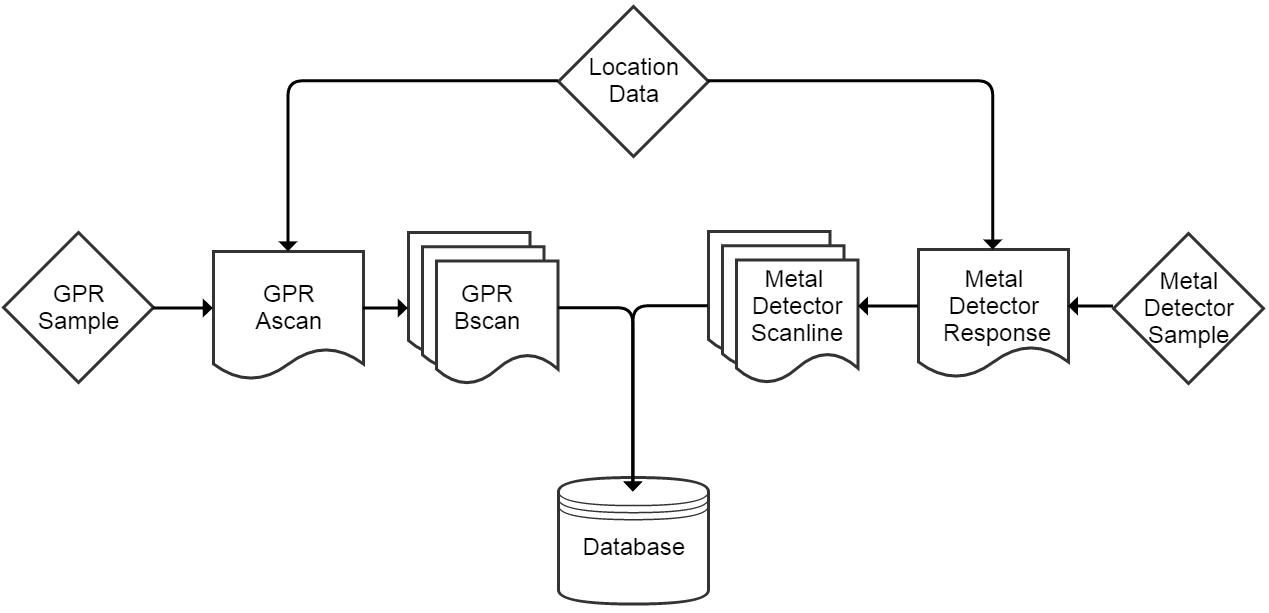
\includegraphics[width=\textwidth]{5-DetailedDesign/data-management.png}
\centering
\caption{Data collection strategy for the signal processing system}
\figlabel{datamanagement}
\end{figure}

The program flow design for the completion of the first detection algorithm is shown in \Figref{agile}. The first algorithm to be attempted is the identification of feature parabolas using the randomised Hough transform over the GPR B-scan, as this method produces a visual output which can easily be tested for correctness by an operator by visual comparison. It will also involve the development of the background signal isolation process, which will also be able to be visually inspected for correctness and will be required for the preprocessing steps of the other detection algorithms.
Once the Feature Parabolas have been isolated from the received signal, criteria will be determined by a human operator which will be used to provide classification between mines and non-mine objects.

\begin{figure}[ht]
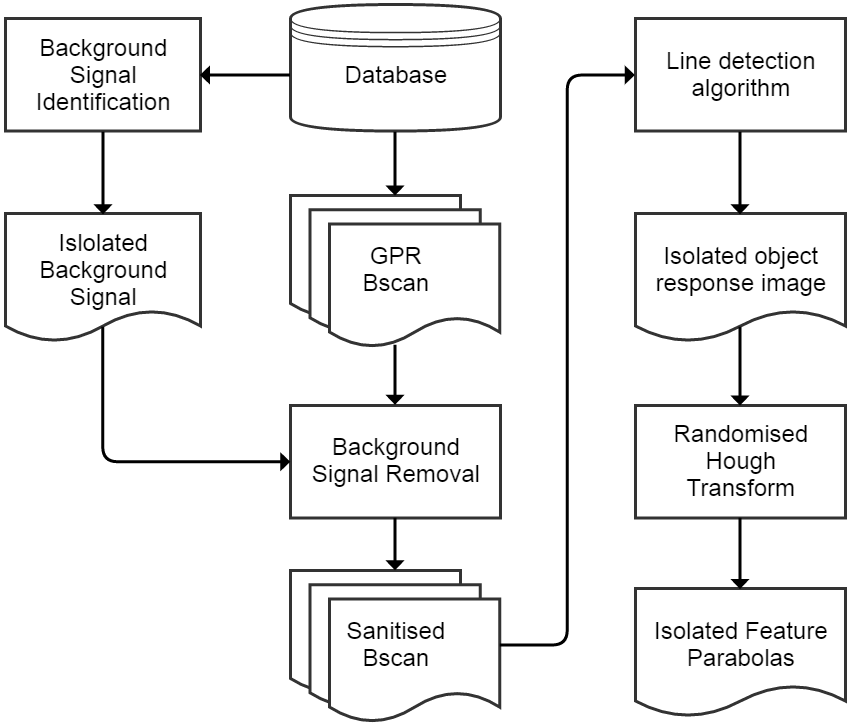
\includegraphics[width=0.8\textwidth]{5-DetailedDesign/agile-strategy.png}
\centering
\caption{Software program flow for initial development stage}
\figlabel{agile}
\end{figure}

\section{Electronics Hardware}
The electronics hardware to be used for the project will fit in the categories as described in the Conceptual Design. The custom electronics work pre-existing on the quad bike supplied by the DSTG meets the requirements for the COTS bespoke electronics, providing digital interfaces to the actuators and sensors attached to the platform. The need for replacement or improvement of any of these electronics will be determined after testing has been completed on the supplied vehicle and their performance has been evaluated.

As the electronics system does not have particularly strict requirements for part selection, and due to the COTS equipment being mostly interchangeable with little effect on appropriateness for the project, the electronics hardware has been chosen on a basis of what is most readily available to the project and most familiar to the project members. This choice reduces time spent in the design stage and allows for a rapid development process to commence as early as possible.

The central processing hardware will be provided by a Windows based desktop computer supplied by the University of Adelaide. A Windows device has been chosen to be able to make use of the provided drivers for the GPR system which are only compatible with 32-bit Windows machines. The selected device has WiFi communications capabilities and dedicated serial communications ports, allowing easy communications to a microcontroller device providing low level I/O.

The microcontroller selected is an Arduino Mega 2560 board, chosen for its cost, availability and fast development time. This board has considerable I/O capabilities that exceed the requirements for the project, but allow for future expansion of sensors and ensures that I/O limitations will not be a concern. The microcontroller will be connected to the desktop computer via the serial port as mentioned above.

\end{document}
































